\section{Exercise 1 - Implement A Benchmark Framework}

The main part of task 1 was to implement a benchmarking framework for the following exercises. This was done succesfully 
and all the demanded quantities where computed and gathered in \texttt{.txt} files named with their respective
 configurations and exercise number. This to postprocess and plot the data within python with low effort. 
 The benchmarking framework is used in exercise 1 with a naive implementation of gathering information of all processes, 
 perform an operation on the gathered information, and distribute the result of the operation to all 
 participating processes. In our case we used the \texttt{MPI\_MAX} operation, which yields the largest 
 element of the buffers. In the following exercises, the same idea is persued (reduce, perform operation, 
 broadcast operation result) but with more sophisticated message passing approaches. 


\begin{figure}[h]
    \begin{center}
        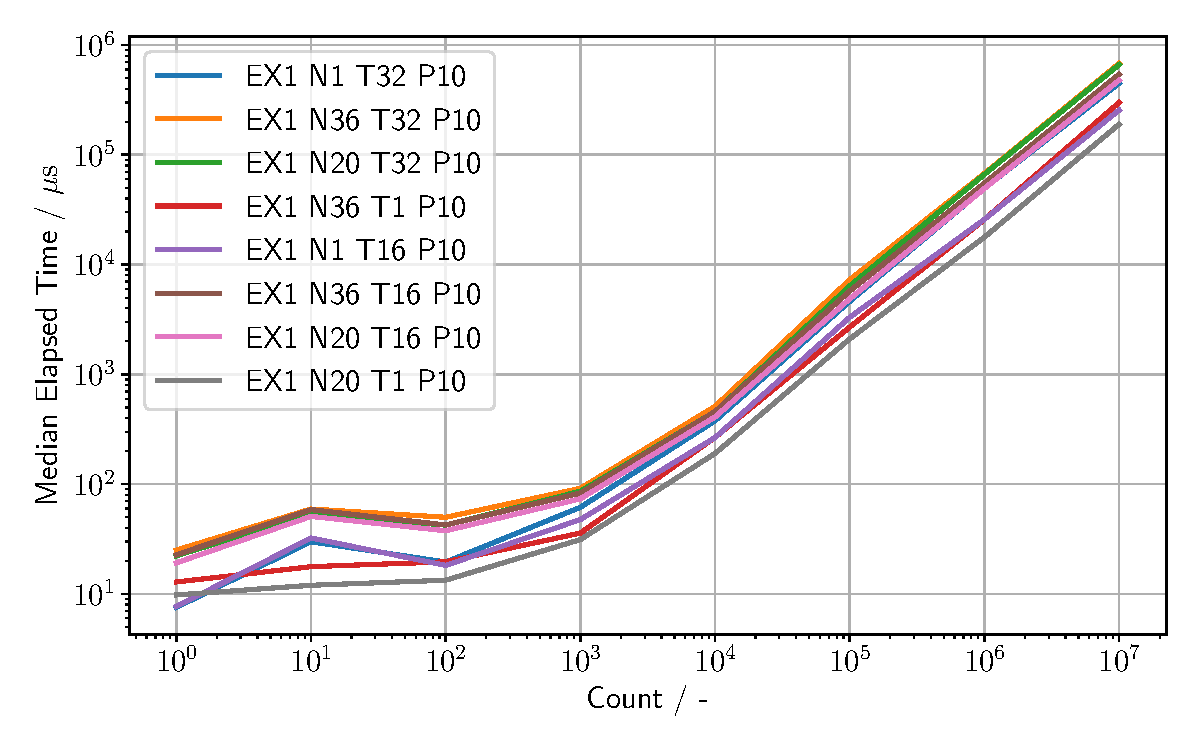
\includegraphics[width=1.0\linewidth]{figures/Ex1_1.pdf}
        \caption{Median Timings for \texttt{MPI\_Reduce + MPI\_Bcast} for all Configurations 
        and powers of 10. Since every \fun{MPI} process performs its own timing, we use 
        \fun{MPI\_Reduce(..,MPI\_MAX)} to retrieve the timing of the slowest process. After 10 Warmup rounds in Ex1 we ran a 100
        iterations to compute the statistic data asked for in Ex1.}
        \label{Ex1_P10_median}
    \end{center}
\end{figure}

For the naive implementation \texttt{MY\_Allreduce()}, which is essentially \texttt{MPI\_Reduce()} followed 
by \texttt{MPI\_Bcast()}, for powers of 10, we observed the timings shown in figure (\ref{Ex1_P10_median}).
The configurations for each measurement are shown in the legend, where N stands for the number of Nodes, T 
for the number of tasks per thread and P is e.g. powers of 10, whereby powers of 10 means that the length 
of the buffers (Count) are all powers of 10.
\begin{figure}[h]
    \begin{center}
        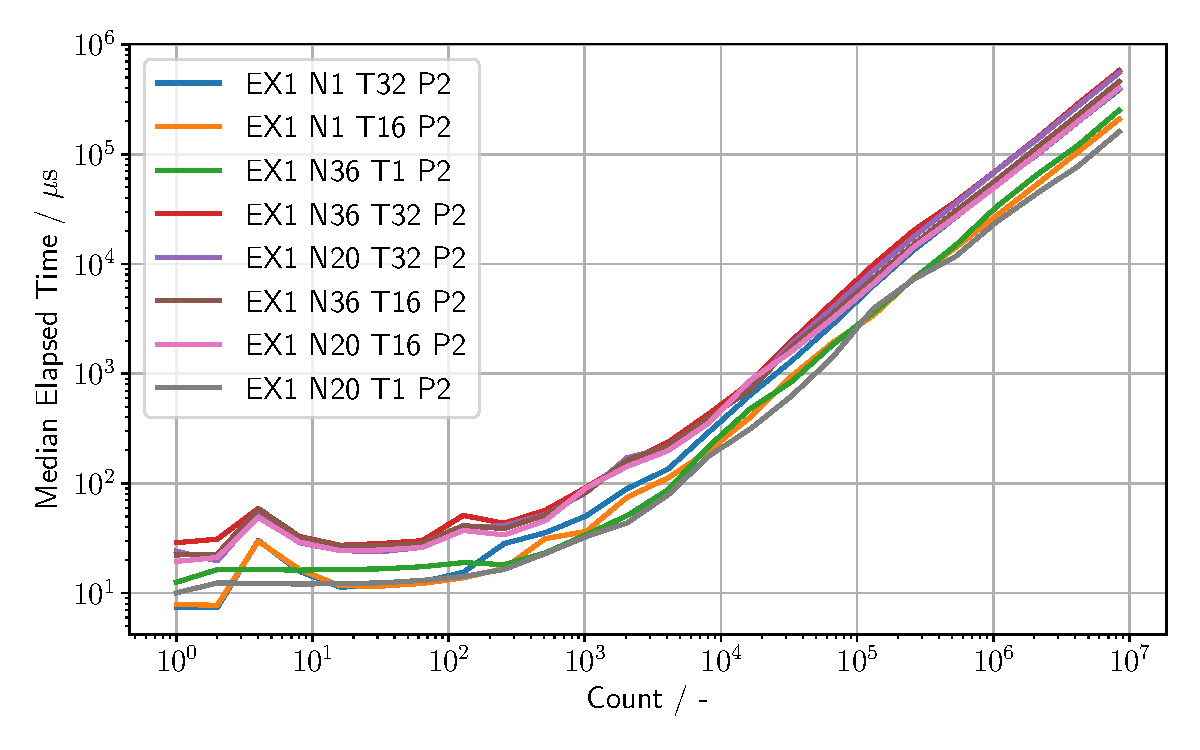
\includegraphics[width=0.8\linewidth]{figures/Ex1_2.pdf}
        \caption{Median Timings for \texttt{MPI\_Reduce + MPI\_Bcast} with all Configurations and powers of 2}
        \label{Ex1_P2_median}
    \end{center}
\end{figure}

\pagebreak

\section{Exercise 2 - Implement Linear Pipeline for \texttt{MPI\_Bcast} and \texttt{MPI\_Reduce}}

The goal of exercise 2 is to implement linear pipelined versions of \texttt{MPI\_Bcast()} and \texttt{MPI\_Reduce()} 
based on the algorithms discussed in the lecture (refer to Algorithm 16 and Algorithm 17 of "Algorithms for Collective 
Communication"). \\

Our implementation for the pipelined reduction -- \texttt{MY\_Reduce\_P()} – aligns with the following idea: We 
distinct between a master process (rank $= 0$), interior processes ($0 <$ rand $<$ size $-1$) and an end process 
(rank $=$ size $-1$). As an output of \texttt{MY\_Reduce\_P()}, the master shall possess the entry-wise maximum as 
reduction result. Additionally, we divide the array that needs to be compared into multiple blocks of size 
\texttt{blockSize} (and probably a smaller block in the end). Goal is to communicate between the processes for each 
block separately. \\

The end process (rank $=$ size $-1$) sends blocks – one after the other -- to the interior process with 
rank $=$ size $-2$. The end process does not receive data, as there are no further processes. Interior processes 
first receive a data block from their neighbor with rank $+1$, perform a local reduction and send this data to their 
other neighbor with rank $-1$. This is repeated for all blocks. The master process receives block data from the interior 
node of rank $=1$.\\

Our implementation for the pipelined broadcast -- \texttt{MY\_Bcast\_P()} – is quite similar to the 
\texttt{MY\_Reduce\_P()} implementation. For broadcast the goal is that the data which is I the beginning 
available for the master process shall be communicated to all the other processes. In order to do so, the master 
process sends its data block wise to its neighbor with rank $=1$ (interior process). Interior processes receive block 
data from their predecessor process and immediately communicate this data to their successor process – block by 
block. The last one to receive the data is the end processor. There is no need to send any further data from here.\\

The trivial combination of \texttt{MY\_Reduce\_P()} and \texttt{MY\_Bcast\_P()} can be seen as a pipelined variant 
of \texttt{MPI\_Allreduce()}.\\

\begin{figure}[h]
    \begin{center}
        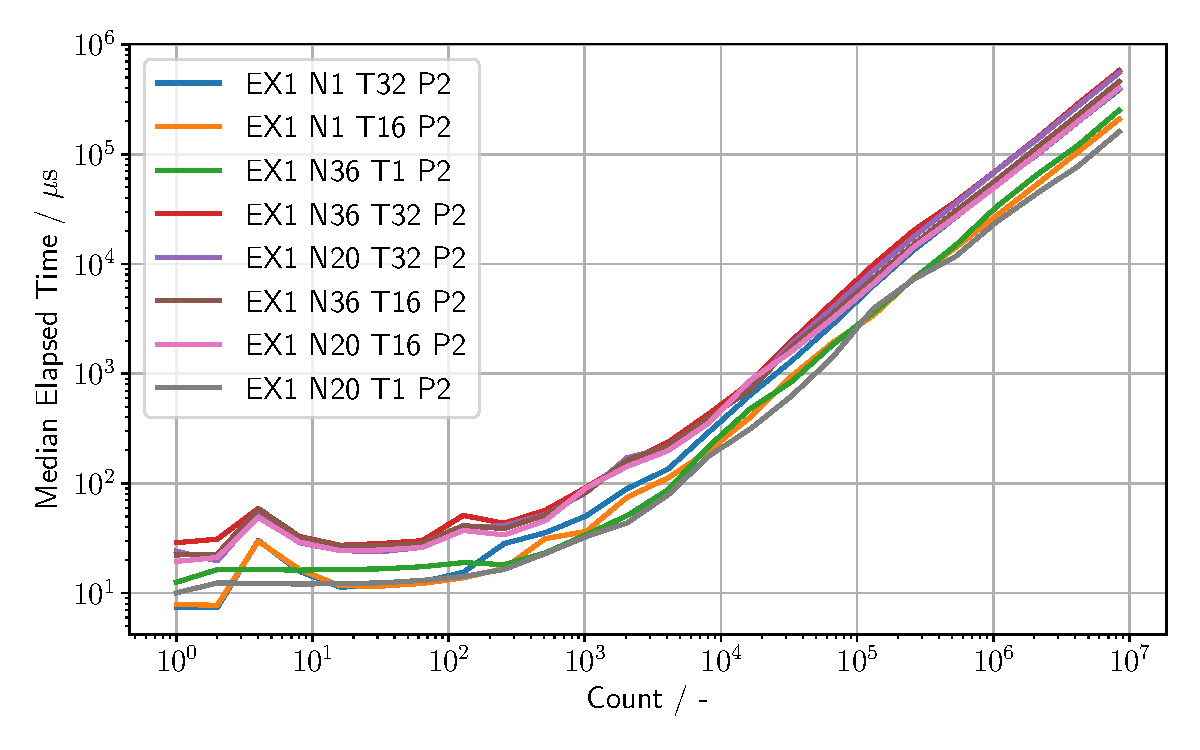
\includegraphics[width=0.3\linewidth]{figures/Ex1_2.pdf}
        \caption{Complete (but unbalanced) binary tree of height $d = 4$ with $p = 9$ nodes.}
    \end{center}
\end{figure}
\pagebreak

\section{Exercise 3 - Combining \texttt{MPI} Processes}
With the goal of saving slightly on communication rounds by combining a pipelined reduction and a 
pipelined broadcast more tightly to keep the processes “more busy”, we end up with the function implementation 
of \texttt{MY\_Allreduce\_P()}. This implementation is completely based on the pipelined tree 
implementation for exercise 5 (REFER HERE TO EX5). For better understanding, refer to exercise 5 first.\\

Hence, we interpret the “lined up” processes as a tree, where each node except one leaf has exactly 
one child and all nodes except the root have a parent node. With this understanding, we reuse the 
implementation of \texttt{MY\_Allreduce\_T()} from exercise 5 by getting rid of the communication between 
a “right child” and it’s parent as in our setting for exercise 3 only “left children” exist.\\

We can expect an improvement compared to the trivial combination of \texttt{MY\_Reduce\_P()} and 
\texttt{MY\_Bcast\_P()}, as in \texttt{MY\_Allreduce\_P()} the reduction already gets started as soon 
as the data of the first block received the master process -- the root node. Therefore, 
$\text{number of processes/nodes} - 1 + \text{number of blocks}$ are needed in \texttt{MY\_Allreduce\_P()}, 
whereas \texttt{MY\_Reduce\_P()} and \texttt{MY\_Bcast\_P()} use $\text{number of blocks}$ communication rounds 
each. For a small numbers of processes/nodes, the number of communication rounds can be reduced based 
on the number of blocks and therefore the blocksize.\\

\pagebreak

